%
% File: results.tex
% Author: Liam O'Shea
% Description: Results
%

\let\textcircled=\pgftextcircled
\chapter{Results, Evaluation \& Conclusion}
\initial{T}his chapter will present and discuss the results produced by the classifiers discussed in the `My Approach' section. Other applications for this work will be suggested and difficulties encountered during the project will be highlighted. Further work can then be discussed within this context. 

\paragraph{Accuracy \& Precision}
Any classification percentages given in this report have been obtained from the average of 5 consecutive results to give an accurate representation of classifier performance. Precision is defined as the degree to which measurements under the same conditions show the same results. Therefore all values have been rounded  to two decimal points since I believe this is more than precise enough for my purposes.

\section {Final results \& Discussion}
Below are the final results for the three best performing classifiers which highlight how the number of eigenvectors used during dimensionality reduction affects accuracy.  
\begin{table}[h]
\begin{center}
    \begin{tabular}{ | l | l | l |}
    \hline
    Classifier & Eigenvectors Used & Accuracy\\ \hline
    SVM & 1 & 72.88\%\\ \hline
    Decision Tree & 1 & 74.58\%\\ \hline
    Neural Network & 1 & 74.60\%\\ \hline
    
    SVM & 2 & 81.36\%\\ \hline
    Decision Tree & 2 & 83.05\%\\ \hline
    Neural Network & 2 & 86.40\%\\ \hline
    
    SVM & 3 & 76.27\%\\ \hline
    Decision Tree & 3 & 79.66\%\\ \hline
    Neural Network & 3 & 79.70\%\\ \hline
    
    SVM & 4 & 86.44\%\\ \hline
    Decision Tree & 4 & {\bf93.22} \%\\ \hline
    Neural Network & 4 & 91.50\%\\ \hline
    
    SVM & 5 & {\bf93.22}\%\\ \hline
    Decision Tree & 5 & 91.53\%\\ \hline
    Neural Network & 5 & {\bf94.90}\%\\ \hline
    
    SVM & 6 & {\bf93.22}\%\\ \hline
    Decision Tree & 6 & {\bf93.22}\%\\ \hline
    Neural Network & 6 & 76.30\%\\ \hline
    
    SVM & 7 & 91.52\%\\ \hline
    Decision Tree & 7 & 91.52\%\\ \hline
    Neural Network & 7 & {\bf94.90}\%\\ \hline
    \hline
    \end{tabular}
\mycaption [Results table for punch classification]{Punch classification accuracy of SVM, Neural Network and Decision Tree on a six class problem.
(Jab, Cross, Left-Hook, Right-Hook, Left-Uppercut, Right-Uppercut)}
\end{center}
\end{table}

{\bf Fig 4.1} shows a summary of all my results pertaining to a different number of eigenvectors and it's effect on different classifiers.
With the exception of using three eigenvectors where all classifiers suffered an accuracy reduction, there follows a general trend that as the number of eigenvectors increases as does the accuracy. This is intuitive since more eigenvectors means the data is represented with increased dimensionality and as such we would expect the SVM to have a small increase in accuracy given more significant data. However since each successive eigenvector represents less variance in the data than the one previously they become a less and less useful way of representing data. 
As the number of eigenvectors increase as does the complexity of classification, since a classifier now has to train on a larger data set which is more costly to compute, resulting in slower running times. If too many eigenvectors are used the classifier will be forced to consider them during training, which for the less significant EVs could result in noise being introduced, making the classifier more prone to over fitting. It will also make feature extraction more difficult.
It is unusual for all three classifiers to experience a drop in accuracy when an extra eigenvector is added, especially one that represents such a large variance in the data. For data this complex I find it surprising that the third eigenvector did not represent meaningful data, however, I can only infer that it instead represents some variance in the data that does not relate to a change in boxing pose.


\begin{table}[h]
\begin{center}
    \begin{tabular}{ | l | l | l |}
    \hline
    Classifier & Eigenvectors Used & Accuracy\\ \hline
    SVM & 6 & 97.83\%\\ \hline
    Decision Tree & 6 & 91.21\%\\ \hline
    Neural Network & 6 & {\bf98.60}\%\\ \hline
    \hline
    \end{tabular}
\mycaption [Results table for good and bad jab classification]{Punch classification accuracy of SVM, Neural Network \& Decision Tree on good \& bad jabs}
\end{center}
\end{table}

SVMs and Neural networks performed excellent on a two-class problem between good and bad jabs {\bf Tab 4.2}. In this case the `bad' jabs were thrown with the elbow sticking out since this is a target characteristic discussed earlier in the background chapter. Given this accuracy we can see that ZeroToHero is capable of distinguishing between very similar poses with only one joint position being significantly different. If this project was extended it is easy to see how this could be used on the other punches to target common beginner mistakes.

\paragraph{Neural Networks}
The neural networks performed excellently, {\bfFig 4.2}, with a surprising drop when using the sixth eigenvector. However, after looking at the behaviour of the other classifiers we can see that it did not change the accuracy of SVM, for neural networks the 7th EV did not change the accuracy. This suggest to me that similar to the 3rd EV it represents some variation that has nothing to do with boxing pose and as such introducing it only reduced accuracy. I believe the decision tree fared better in this case due to the fact that it is very robust to errors, both in classification and training.\clearpage

\begin{figure}[h]
    \centering
    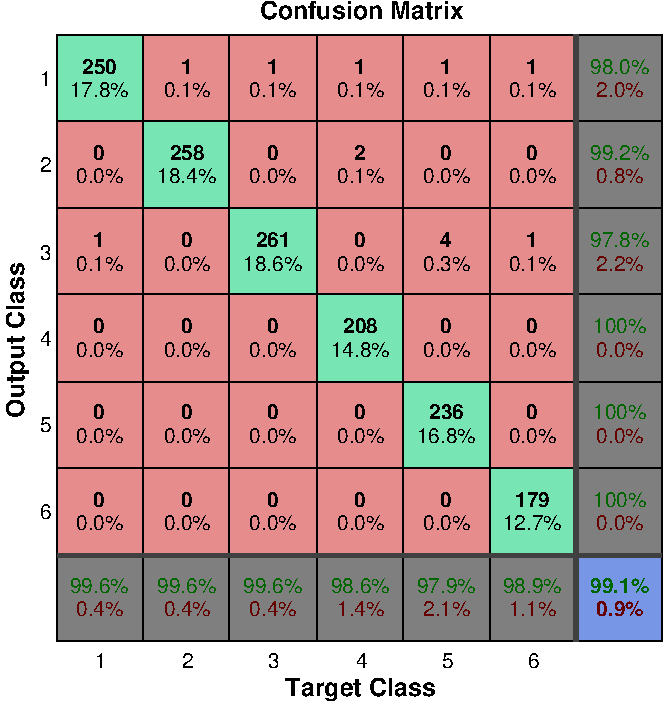
\includegraphics[height=0.25\textheight]{fig05/CMtrain-crop.pdf}
    \mycaption[Neural network confusion matrix on training set]{Neural network confusion matrix on training set}
    \label{fig:drcomp}
\end{figure}

\begin{figure}[h]
    \centering
    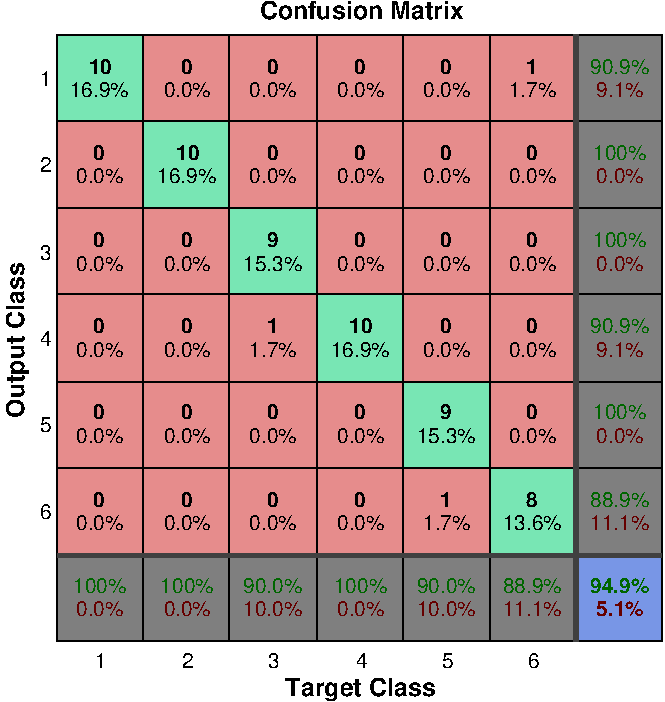
\includegraphics[height=0.25\textheight]{fig05/CMtest-crop.pdf}
    \mycaption[Neural network confusion matrix on a test set]{Neural network confusion matrix on a test  of 10 of each punch.}
    \label{fig:drcomp}
\end{figure}

\begin{figure}[h]
    \centering
    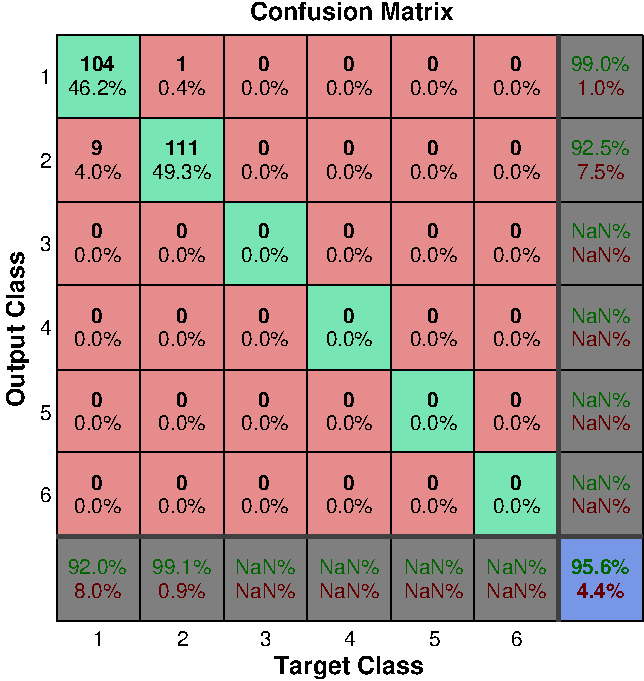
\includegraphics[height=0.25\textheight]{fig05/2classcm-crop.pdf}
    \mycaption[Neural network confusion matrix on a two-class problem]{Neural network confusion matrix on a two-class problem}
    \label{fig:drcomp}
\end{figure}

\section{Difficulties}
I found this project to be an excellent way to combine my interest in boxing with my Computer Science background. It was however a difficult project and I ran into a few problems during research and development.
One of the first difficulties is that skeleton data is can be incredibly noisy. After collecting datasets from both local clubs and the university boxing club I discovered that it was incredibly difficult, with my current system, to link these sequences together and to then use them as one large training set. Even though I had taken precautionary measures such as asking all of my subjects to stand in approximately the same spot during recording, even slight variations in distance from the Kinect combined with different body types resulted in unusable data. 
Different body types affected the speed at which punches were thrown since a short stocky person or a particularly tall person might be slower than average. This resulted in a different time series, but this can be successfully dealt with by the current implementation.
I found differences in distance from the Kinect during recording made a big difference, as did skeletal height. As arm length tends to be proportional to skeletal height, those with longer arms had a shorter distance between themselves and the kinect after the punch has been delivered. Conversely those with shorter arms had a longer distance.
Since the current system uses skeletal joint co-ordinates the projection coefficient for the first component is heavily influenced by distance from the Kinect. Unsurprisingly this meant my data was un-normalised, which made it difficult to spot patterns that could have been used to classify the punches. It also made it almost impossible to automatically segment since the projection coefficients for the first principal components were quite different even within punches of the same class {\bf Fig 4.4}.

\begin{figure}[h]
\centering
\begin{minipage}{8.0cm}
    \centering
    \subtop[]{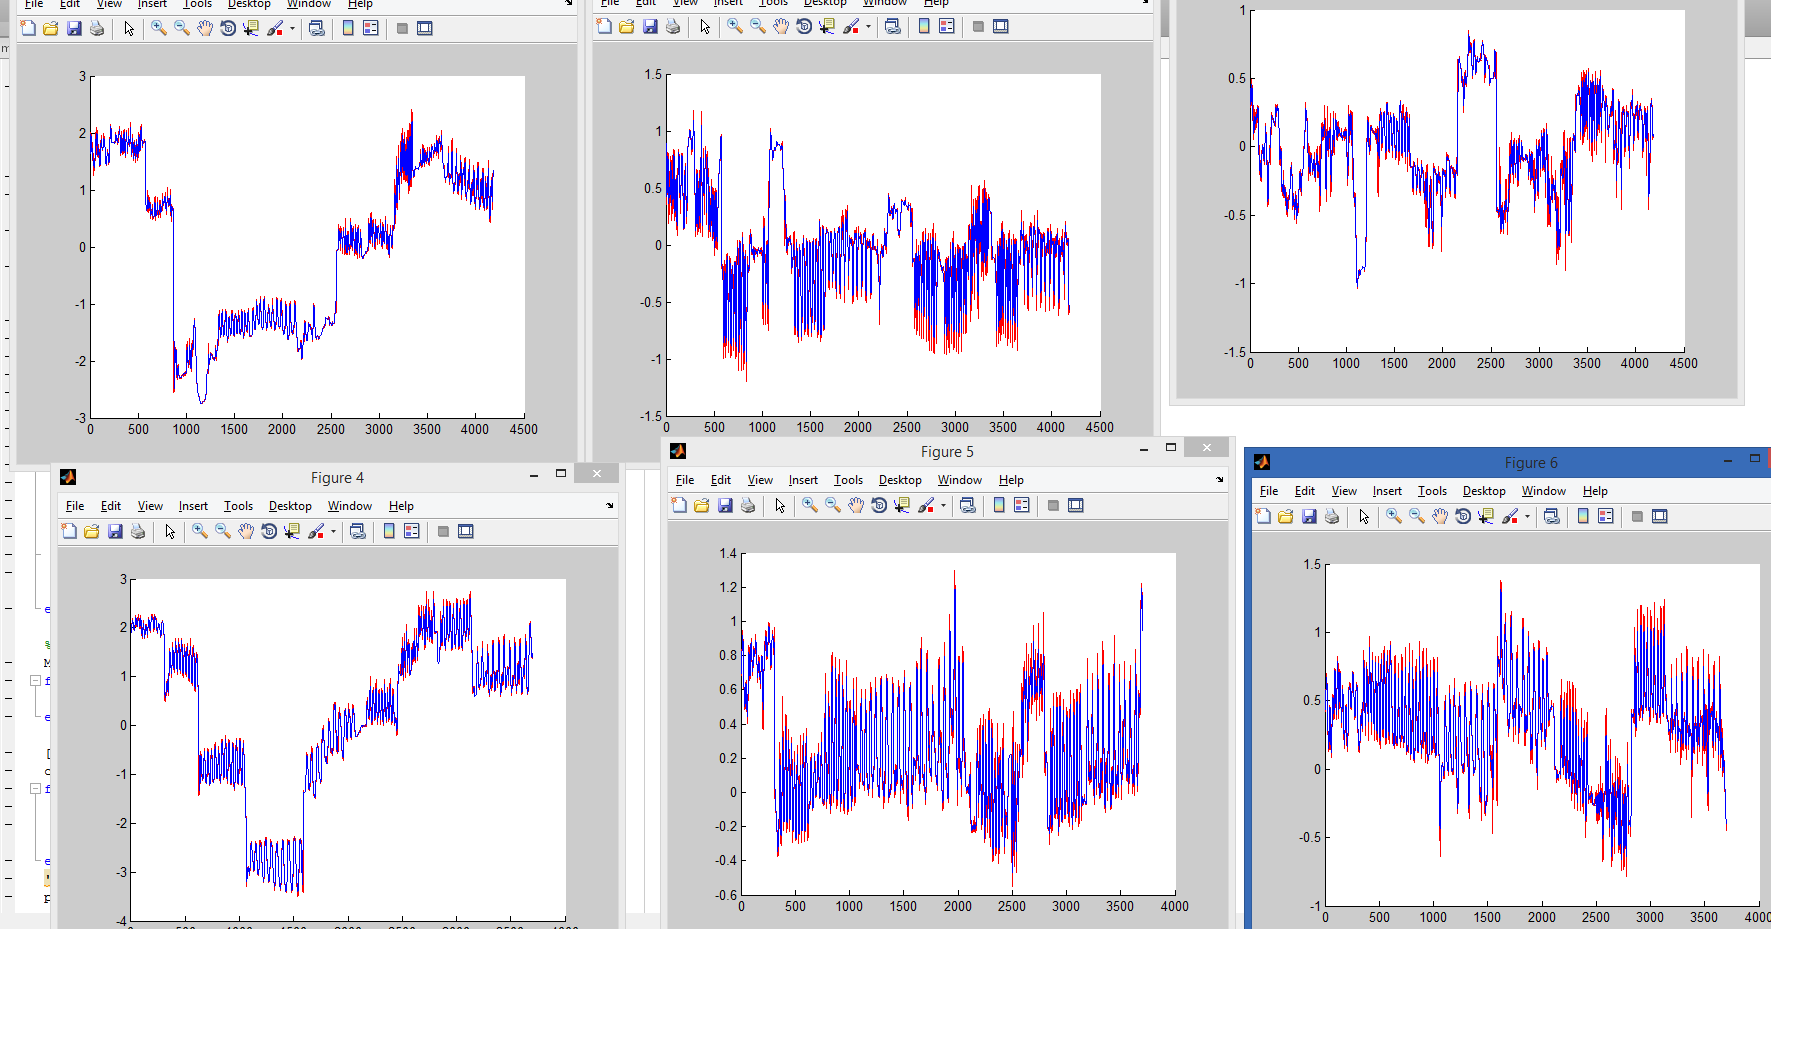
\includegraphics[height=0.25\textheight]{fig05/fullnonorm}}
    \label{fig:1}
\end{minipage}
\vspace{2.0cm}
\qquad
\begin{minipage}{8.0cm}
    \centering
    \subtop[]{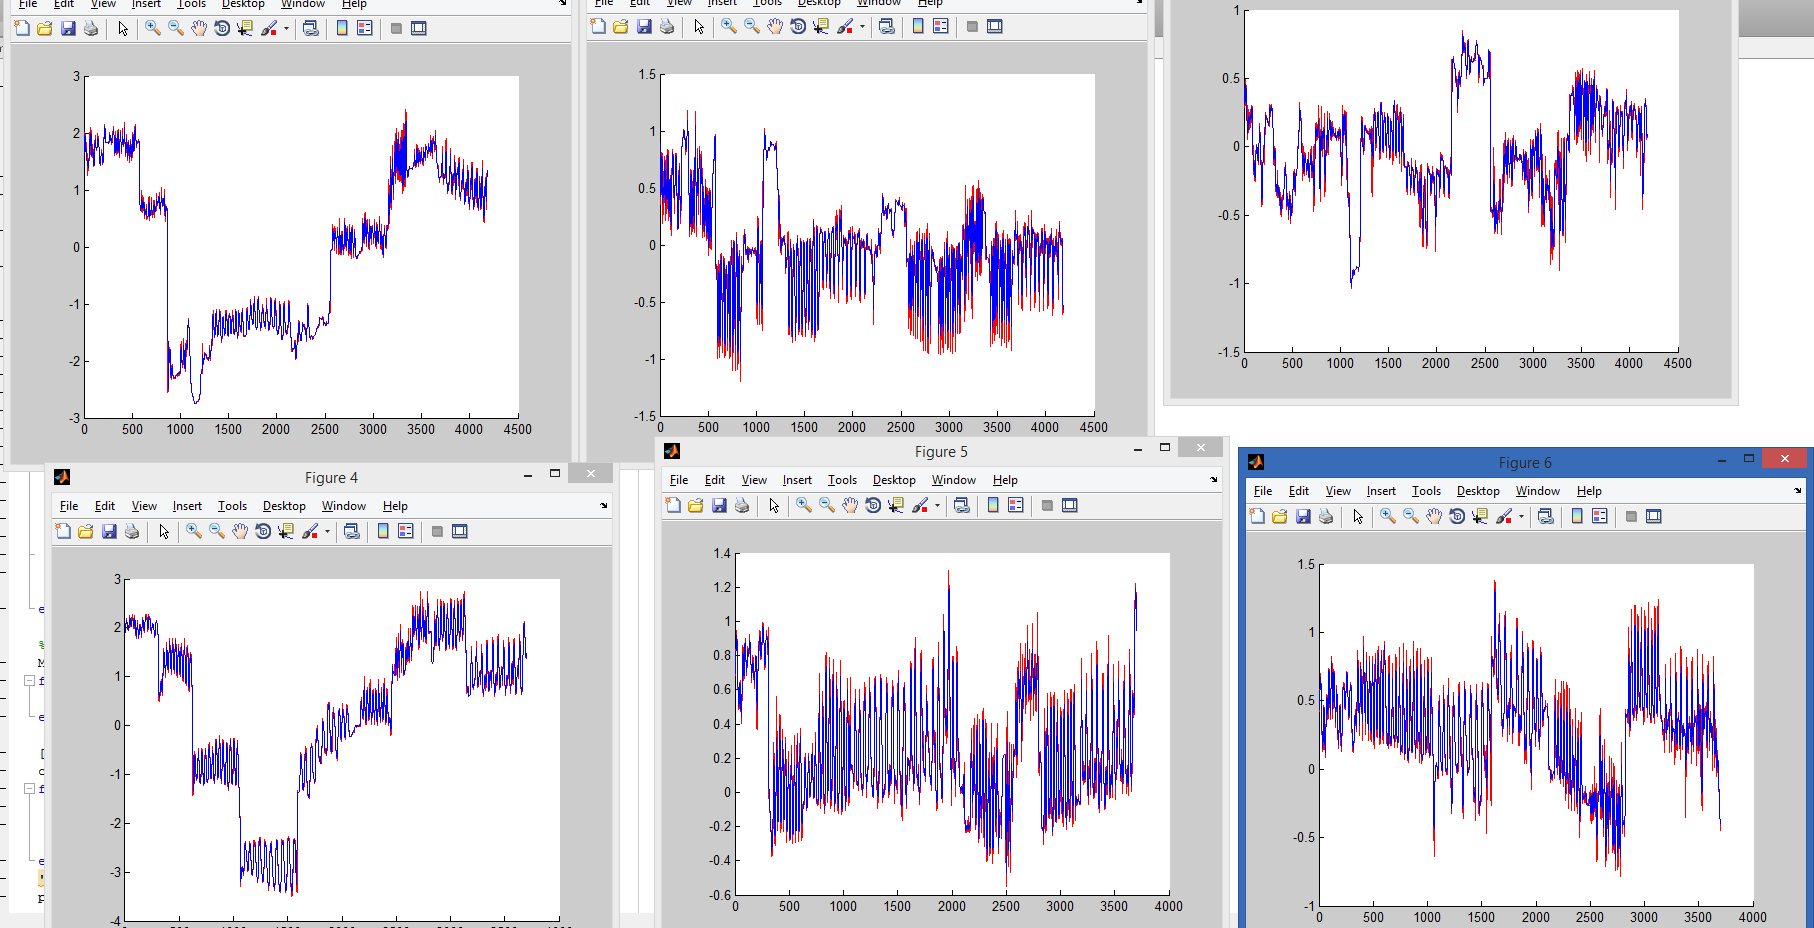
\includegraphics[height=0.25\textheight]{fig05/fullnonorm2}}
    \label{fig:2}
\end{minipage}
\mycaption[Un-normalised punch sequences] {Twelve different un-normalised punch sequences. Given that these are sequences of the same punch you would expect them to be reasonably similar, however, the `jumps' in value on the y-axis are where un-normalised data has been joined together. This demonstracted the diffenece that the distance from the Kinect can make during the recording stage. (The `jumps' on the y-axis correspond to distance in the z direction from the Kinect during recording.)}
\end{figure}


\subsection{Normalisation}
In an attempt to normalise my data for future recording sessions I took the the central hip joint and used this as the skeletal centroid, with it being given position (0,0,0). This resulted in all joints being given positions relative to the hip joint. `Movement' has two components; the global translation of the skeleton and movement in the pose itself. By normalising on the hip joint the global movement is removed which is useful since we are only interested in a change of pose. Although this method seemed to reduce noise and improve my classification, I still had the problem that the first principal component was heavily influenced by distance from the Kinect.

\subsection{Further Work \& Improvements}
My first improvement would be to develop an algorithm for normalising skeleton data so that data from multiple recording sessions and distances from the Kinect could be used together as one dataset. Using the above hip normalisation technique it would be possible to look at the distance from each joint to the centroid and normalise those values based on a `normal' base value and scaling according. This would be useful in accounting for different lengths of limbs and body types. 

I would also like to implement a system where distance from the Kinect was unimportant. This could be by using velocity and implementing a better segmentation algorithm or using quaternions and their associated rotation matricies instead of joint position.

Although the system is fast enough to perform in real time it is currently not `live' since data is recorded and then analysed, this would be the next step. 

Finally I would like to assess the quality of every punch, currently we can classify a punch and tell if it is a good or bad punch. I would link both classifiers together, possibly using an ensemble method so each punch is recognised and then assessed on it's quality based on the classification.

\subsection{Other Applications}
Makaton is language program that uses gestures, body language, signs and symbols to communicate, designed for individuals that struggle to communicate via speech \cite{MAKATON} \cite{MAKATONwiki}. For Makaton to work effectively you must be facing those you are trying to communicate with while repeating simple gestures with your hands. This shares similarities with this system since you must also be relatively face-on and the movement is periodic. I believe this system could be adapted relatively quickly and easily to recognise Makaton gestures. For similar reasons this could also be used to recognise British Sign Language (BSL) although this would be more complicated than the very simple gestures that Makaton relies on.

\begin{figure}[h]
\centering
\begin{minipage}{7.0cm}
    \centering
    \subtop[]{
\includegraphics[height=0.25\textheight]{fig05/maka1}}
    \label{fig:1}
\end{minipage}
\vspace{2.0cm}
\begin{minipage}{7.0cm}
    \centering
    \subtop[]{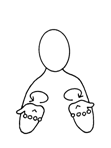
\includegraphics[height=0.25\textheight]{fig05/maka2}}
    \label{fig:2}
\end{minipage}
\mycaption[Makaton gestures] {Examples of simple gestures that make up the Makaton language}
\end{figure}

ZeroToHero could also be used to classify any atomic activity \cite{Aggarwal2007} which can be temporally segmented such as kicking, punching, jumping as well as sitting and standing. 

It could be used in the field of Human-Computer interaction for simple gesture recognition provided the gestures were designed with Kinect's limitations in mind. A simple semaphore-type system would be ideal since the gestures would be reasonably easy to recognise provided they were repeated.

Finally my system could be incorporated into pre-existing martial arts trainers to add additional functionality or to simply improve their current punch recognition algorithm.

\paragraph{Conclusion}
I have presented a real time punch recognition and quality assessment algorithm which has the potential to bring specialist boxing coaching into a home environment. Human poses were recorded using the Kinect \& Microsoft SDK, an already widespread, low cost consumer device with high accessibility. 
I investigated the efficacy of a number of dimensionality reduction techniques when applied to pose sequences including CCA, LLE, Hessian LLE, Laplacian Eigenmaps, LTSA and PCA. I found that PCA was most suitable for facilitating time series segmentation since I could consistently obtain a sinosidal-like sequence. This enabled me to perform automatic punch segmentation on the reduced dimensionality pose-time series and extract useful features from the original unsmoothed reduced dimensionality data set. Segmentation was achieved by smoothing the projection coefficients for the first principal components, before extracting local maxima from across the time series. Each maxima was then inspected by a set of heuristics which determine whether it signifies the start of a punch or is just a local maxima that still exists after smoothing.
Finally, the optimal number of principal components retained and the suitability of a variety of classifiers were empirically assessed including SVM, Neural Networks(NN) and Decision trees(DT). On a 6 class problem of punch classification, ZeroToHero achieved accuracy results of {\bf 94.90\%} with NN and {\bf 93.22\%} using SVM and DT. On a two-class problem of good and bad jabs, an accuracy of {\bf 98.60\%} was achieved using NN, {\bf 97.83\%} by SVM and {\bf 91.21\%} by DT.